\documentclass{article}

\usepackage[a4paper,top=20mm,bottom=20mm,left=20mm,right=20mm,nohead,nofoot]{geometry}

\usepackage{comment}
\usepackage{amsmath}
\usepackage{amstext}
\usepackage{amsfonts}
\usepackage{amssymb}
\usepackage{graphicx}

\begin{document}

\title{IS and graph measures}
\author{\'Oscar Godoy, Jos\'e A. Langa,  Jos\'e R. Portillo and Fernando Soler-Toscano}
\maketitle{}

\section{Introduction}
\label{sec:introduction}

Explain the methodology. IS measures on the COMA paper and graph
measures (JoseRa).

How the 200 random alphas are built. There is only one or two negative
values in each $\alpha$. The values are randomly picked from a normal
distribution and then the resulting vector is normalised. 

\section{Simulation of biological networks}
Normal, Exponential, Logistic, Geometric, Poissson, Negative binomial.

Kolmogorov-Smirnov test with bootstrapping number $10000$ (Table~\ref{tab:ksboot}).
\begin{table}[hbtp]

    \centering
    \begin{tabular}{|l|c|c|c|c|c|c|}
        \hline
         P-Value & Normal & Exponential & Logistic 
         & Geometric & Poissson & Negative binomial\\ \hline
         Mean & 0.006944 & 0.0006944 & 0.0037904 
         & 0.0214488 & 0.0048432 & 0.5143584 \\ \hline
         $\ge 0.5$ (\%) & 0.8 & 0 & 0 & 1.6 & 0 & 58.4  \\ \hline
         $\ge 0.5$ (\#) & 1 & 0 & 0 & 2 & 0 & 73  \\ \hline
    \end{tabular}
    \caption{Kolmogorov-Smirnov test with bootstrapping number $10000$.}
    \label{tab:ksboot}
\end{table}


\section{Graph measures}

undirected, directed, weighted measures

order, size, number of triangles, 
mean degree, mean degree of the neighbourgh?? knn, 
diameter, diameter no weighted,
modularity, modularity no weighted,
mean of closeness centrality, mean of harmonic centrality, 
centrality of betweenness,centrality of betweenness by edges,
eigenvalue centrality, 

\subsection{transitivity, mean of the local transitivity, mean of the Barrat transitivity,}

sacado del manual de igraph--R


Note that there are essentially two classes of transitivity measures, one is a vertex-level, the other a graph level property. Transitivity measures the probability that the adjacent vertices of a vertex are connected. This is sometimes also called the clustering coefficient.

Types of the transitivity  

hay varios modos de calcularla, pero están correlados (o lo estaban en los grafos de poisson, hay que mirar eso también)

"global" The global transitivity of an undirected graph. This is simply the ratio of the count of triangles and connected triples in the graph. In directed graphs, edge directions are ignored.

"local" The local transitivity of a vertex is the ratio of the count of triangles connected to the vertex and the triples centered on the vertex. In directed graphs, edge directions are ignored.

"barrat" The weighted transitivity as defined by A. Barrat. See details below.


There are several generalizations of transitivity to weighted graphs, here we use the definition by A. Barrat, this is a local vertex-level quantity, its formula is

$$
C_i^w=\dfrac{1}{s_i(k_i-1)}
\Sigma_{j,h}\dfrac{w_{ij}+w_{ih}}{2}a_{ij}a_{ih}a_{jh}
$$

$s_i$ is the strength of vertex $i$, i.e., the sum of the edge weights of the adjacent edges for each vertex. , $a_{ij}$ are elements of the adjacency matrix, $k_i$ is the vertex degree, $w_{ij}$ are the weights.

This formula gives back the normal not-weighted local transitivity if all the edge weights are the same.

The barrat type of transitivity does not work for graphs with multiple and/or loop edges. If you want to calculate it for a directed graph, call as.undirected with the collapse mode first.

Wasserman, S., and Faust, K. (1994). Social Network Analysis: Methods and Applications. Cambridge: Cambridge University Press.

Alain Barrat, Marc Barthelemy, Romualdo Pastor-Satorras, Alessandro Vespignani: The architecture of complex weighted networks, Proc. Natl. Acad. Sci. USA 101, 3747 (2004)



\subsection{diversity}

The diversity of a vertex is defined as the (scaled) Shannon entropy of the weights of its incident edges:
nosotros calculamos la diversidad media

Nathan Eagle, Michael Macy and Rob Claxton: Network Diversity and Economic Development, Science 328, 1029–1031, 2010.

es interesante porque introduce el concepto de entropía
habría que comprobar si los vértices de grado dos o menos afectan al cálculo, eso no está hecho


%data.frame(orden=orden,tamano=tamano,numtriangulos=triangulosS,
%  sumgrados=sumagrados,
%  mediagrados=mediagradosS,diametro=diametro,
%  mmmgradovecinos=mediamediagradovecinos,modularidad=modularidad,
%  modNP=modularidadNP,
%  centcercania=mediacercania,centarmonica=mediaarmonica,
%centintermediacion=intermediacion,centintermediacionaristas=intermediacionaristas,
%  diametroS=diametroS,
%  centcercaniaS=mediacercaniaS,centarmonicaS=mediaarmonicaS,
% centintermediacionS=intermediacionS,centintermediacionaristasS=intermediacionaristasS,
%  centAutovalor=autovalorS,
%  transitividad=transitividad,
%  transitividadmlocal=mediatransitividadlocalS,
%  transitividadmbarrat=mediatransitividadbarratS,
%  diversidad=diversidadS

\section{Generating \emph{artificial, syntetical} networks}

\section{Comparing all IS with different $\alpha$ values}
\label{sec:comparing-all-with}


\begin{figure}[htbp!]
  \centering{}
  % chart.Correlation(cor(redes1000data[,c(4,5,9,16,17,19,23,31)], method="spearman"),2)
  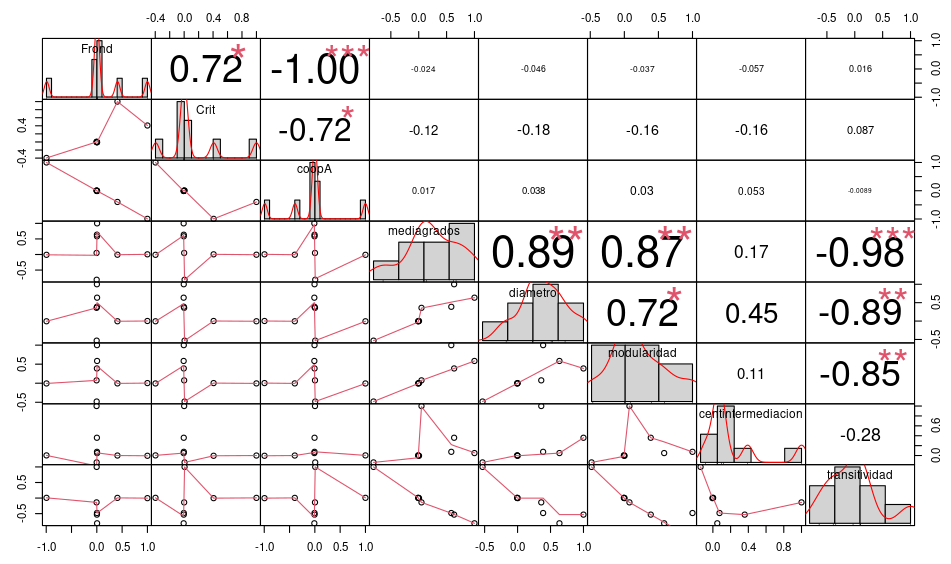
\includegraphics[width=8cm]{img/correlRedes1000}
% chart.Correlation(cor(redesS1000data[,c(4,5,9,16,17,19,23,31)], method="spearman"),2)
  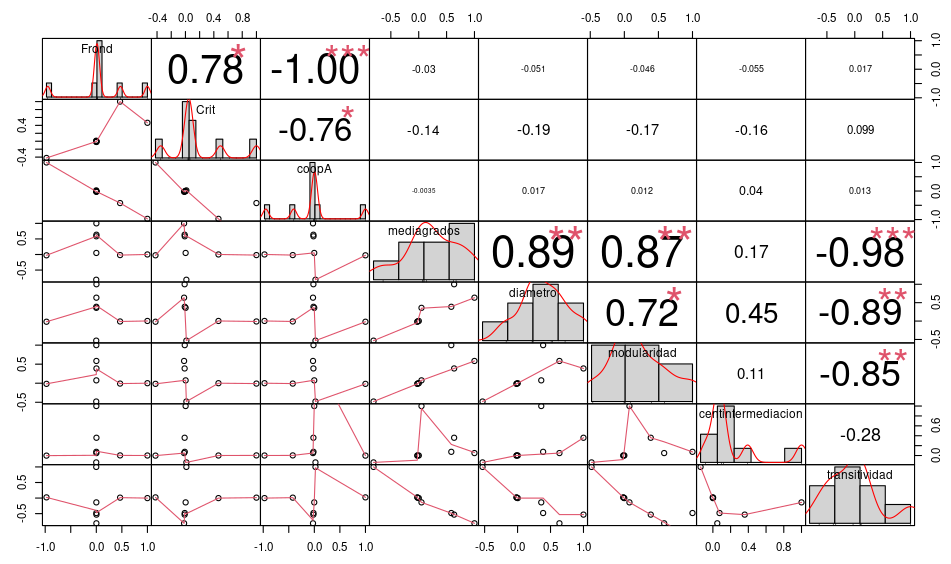
\includegraphics[width=8cm]{img/correlRedesS1000}\\
% chart.Correlation(cor(filter(redes1000data,coopA > 0)[,c(4,5,9,16,17,19,23,31)], method="spearman"),2)
  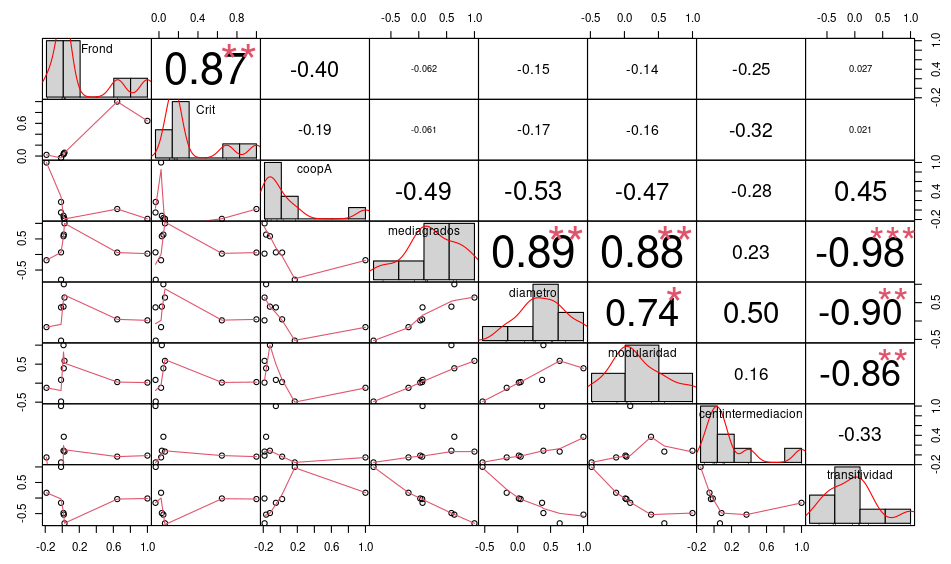
\includegraphics[width=8cm]{img/correlRedes1000CoopMay0}
% chart.Correlation(cor(filter(redesS1000data,coopA > 0)[,c(4,5,9,16,17,19,23,31)], method="spearman"),2) 
  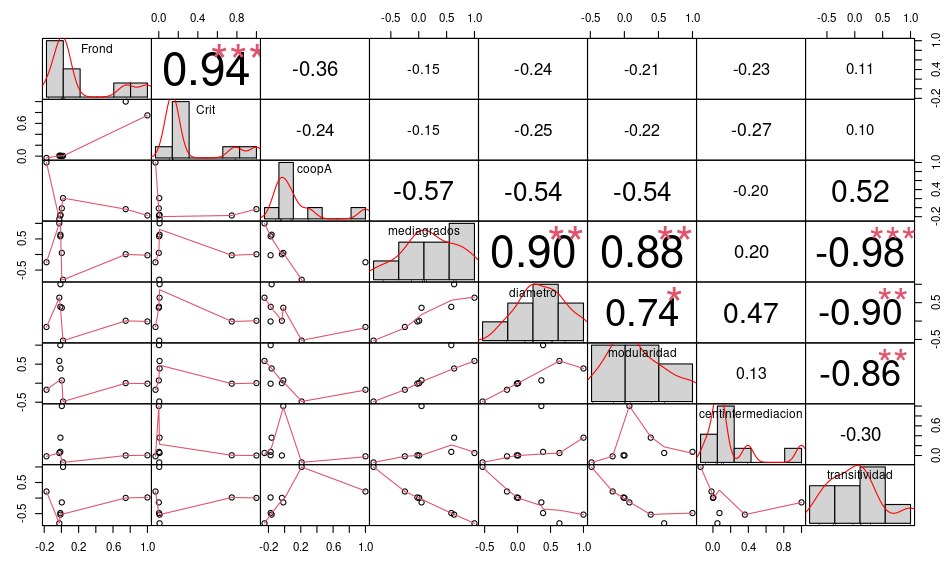
\includegraphics[width=8cm]{img/correlRedesS1000CoopMay0}
  \caption{Correlation of IS and GR measures for 1000 random $7$-node
    networks with 200 random $\alpha$ values. The top row shows the
    correlations for 1000 random networks (left) and their symmetric
    versions (right) of some IS and GR measures. The bottom row shows
    the correlations of the same graphs but only for the IS with a
    coopA value greater than 0.}
  \label{fig:redes1000allAlphas}
\end{figure}

\begin{figure}[htbp!]
  \centering{}
% ggplot(data = filter(redes1000data, coopA >= 0)) +
%   geom_point(mapping = aes(x = modularidad, y = coopA), position =
%   "jitter") 
  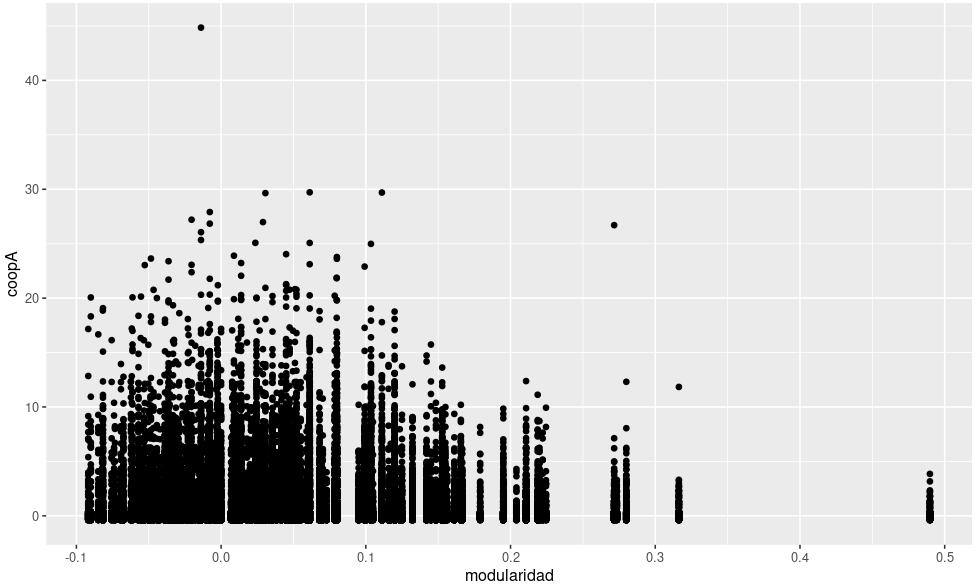
\includegraphics[width=6cm]{img/coopMod1000AllA}\quad\quad
%  ggplot(data = filter(redesS1000data, coopA >= 0)) +
%  geom_point(mapping = aes(x = modularidad, y = coopA), position =
%  "jitter")
  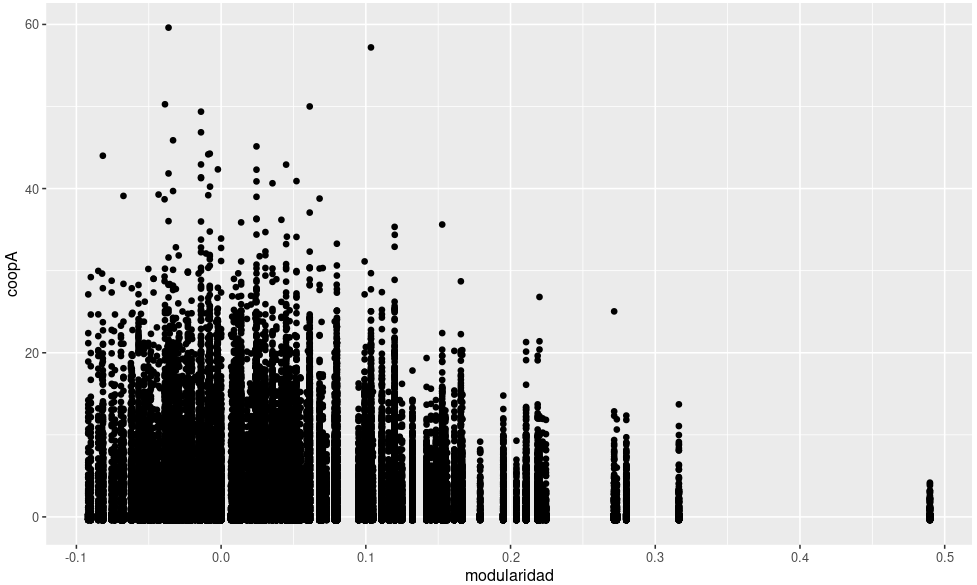
\includegraphics[width=6cm]{img/coopModS1000AllA}
  \caption{Modularity and cooperation in 1000 random graphs. Left:
    Non-symmetric. Right: Symmetric.}
  \label{fig:modCoop1000RandA}
\end{figure}

There are no relevant correlations by looking at all $\alpha$
values. This is in line to what we know about cones, each $\gamma$
matrix produces several cones, there are $\alpha$s in each cone, and
according to them different ISs are produced. See
Fig.~\ref{fig:redes1000allAlphas}. Moderate correlations appear
between cooperation and some graph measures by looking only at those
IS with a cooperation value greater than
0. Fig.~\ref{fig:modCoop1000RandA} shows the relation of cooperation
and modularity. 

\section{Looking at single $\alpha$ values}
\label{sec:looking-at-single}


\begin{figure}[htbp!]
  \centering{}
  % chart.Correlation(cor(filter(redesS1000data,coopA > 0 & nAlpha ==
  % 7)[,c(4,5,9,16,17,19,23,31)], method="spearman"),2) 
  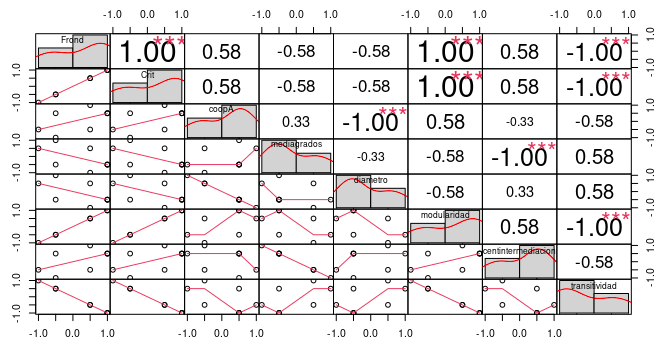
\includegraphics[width=7cm]{img/corrS1000A07}\quad\quad
  % chart.Correlation(cor(filter(redesS1000data,coopA > 0 & nAlpha ==
  % 10)[,c(4,5,9,16,17,19,23,31)], method="spearman"),2) 
  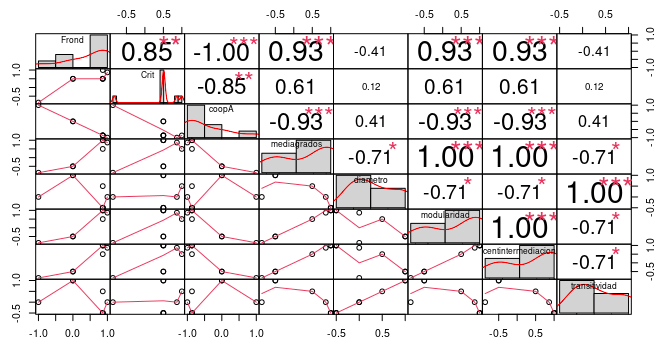
\includegraphics[width=7cm]{img/corrS1000A10}
  \caption{Correlation of IS and GR measures for a single $\alpha$
    value. The 1000 random symmetric graphs are used. Left:
    Correlation of measures for $\alpha = (-0.21, 0.36, -0.29, 0.2, 0.61, 0.06, 0.58)$. Right: Correlation for
    $\alpha = (-0.22, 0.07, 0.19, 0.73, 0.48, -0.22, 0.32)$.}
  \label{fig:corrDiffAlphas}
\end{figure}


\begin{figure}[htbp!]
  \centering{}
  % ggplot(data = filter(redesS1000data, nAlpha == 11)) +
  % geom_point(mapping = aes(x = modularidad, y = coopA), position =
  % "jitter") 
  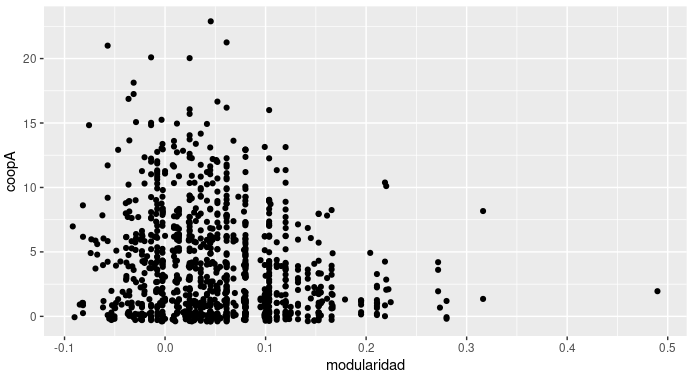
\includegraphics[width=7cm]{img/coopModS1000A11}\quad\quad
  % ggplot(data = filter(redesS1000data, nAlpha == 15)) +
  % geom_point(mapping = aes(x = modularidad, y = coopA), position =
  % "jitter") 
  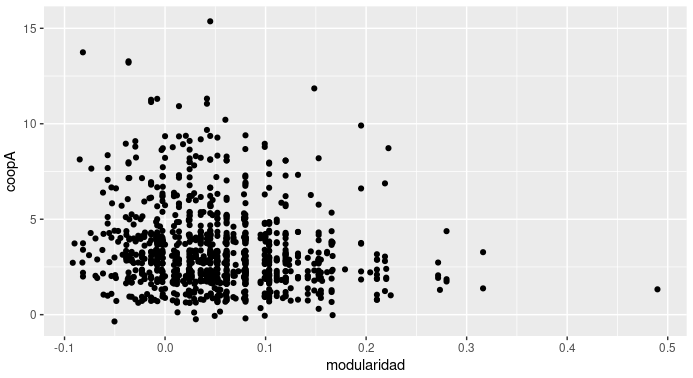
\includegraphics[width=7cm]{img/coopModS1000A15}
  \caption{Modularity and cooperation in 1000 random symmetric graphs
    with a fixed $\alpha$ value. Left: $\alpha = (-0.05, 0.66, 0.22,
    0.64, -0.18, 0.19, 0.17)$. Right: $\alpha = (0.63, -0.02, 0.27,
    0.55, 0.27, 0.15, -0.37)$.} 
  \label{fig:coopModS1000DiffAlphas}
\end{figure}

\begin{figure}[htbp!]
  \centering{}
  % ggplot(data = filter(redesS1000data, nGraph >= 1 & nGraph <= 200 &
  % nAlpha >= 11 & nAlpha <= 15)) +
  % geom_point(mapping = aes(x = nGraph, y = coopA, color = nAlpha),
  % position = "jitter")
  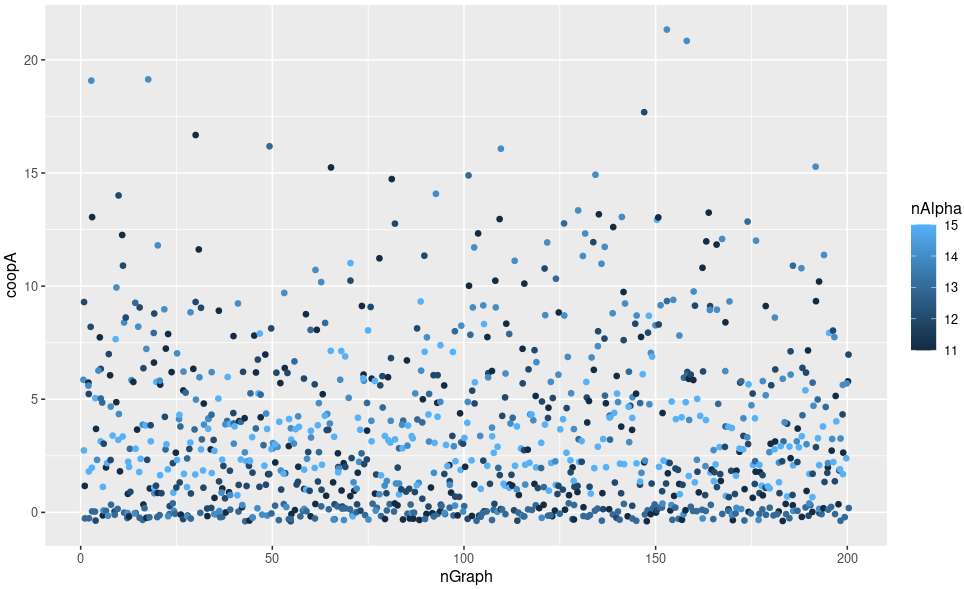
\includegraphics[width=7cm]{img/coopDistS200A11to15}\quad\quad
  % ggplot(data = filter(redesS1000data, nGraph >= 1 & nGraph <= 200 &
  % nAlpha >= 11 & nAlpha <= 15)) + 
  % geom_point(mapping = aes(x = nGraph, y = Frond, color = nAlpha),
  % position = "jitter") 
  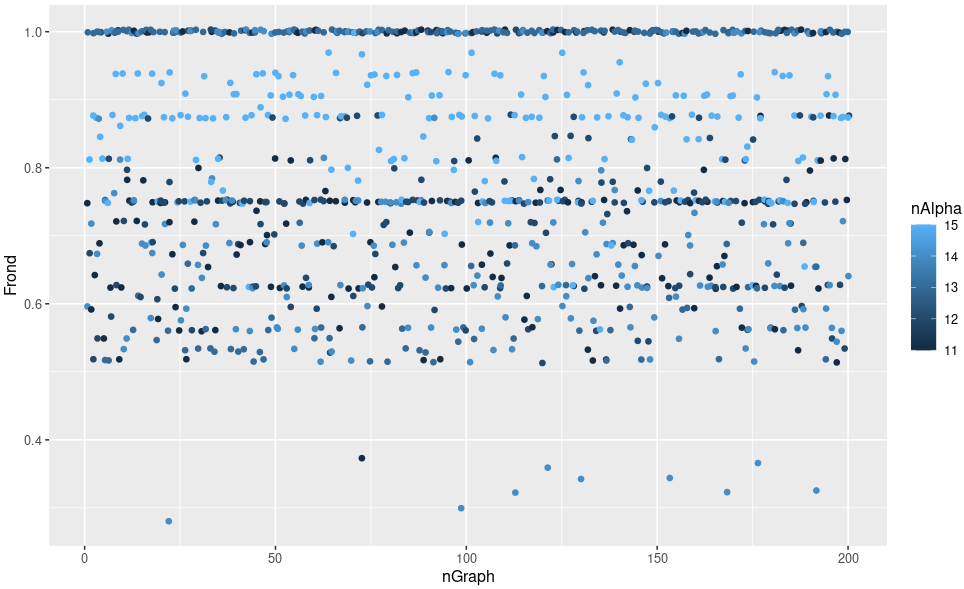
\includegraphics[width=7cm]{img/frondDistS200A11to15}
  \caption{Distribution of cooperation A (left) and frondosity (right)
    values for 200 random symmetric graphs with five different
    $\alpha$ values.} 
  \label{fig:coopDistS200A11to15}
\end{figure}

  Given a single $\alpha$, some correlations among IS and GR
  measures may appear, but they change by looking at different
  $\alpha$ values (Fig.~\ref{fig:corrDiffAlphas}). Correlations depend on
  which nodes have the negative values, or specific features of the
  chosen $\alpha$ (Fig.~\ref{fig:coopDistS200A11to15}). 

\section{Mean value of each graph}

\begin{figure}[htbp!]
  \centering{}
  % chart.Correlation(cor(redes100groupNonCW[,c(2,3,4,5,6,7,8,9,10)],
  % method="spearman"),2)
  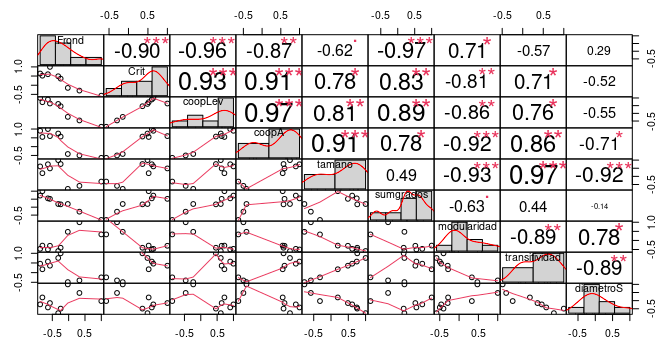
\includegraphics[width=8cm]{img/corrISGR100NonCW}\quad\quad
  % chart.Correlation(cor(redesS100groupNonCW[,c(2,3,4,5,6,7,8,9,10)],
  % method="spearman"),2)
  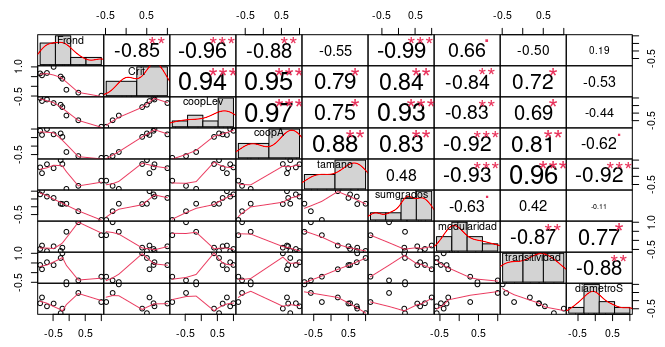
\includegraphics[width=8cm]{img/corrISGRS100NonCW}
  \caption{Correlation of IS and GR measures of 100 random graphs with
  different sum of edge weights. Left: non-symmetric. Right: symmetric.}
  \label{fig:corr100nonCW}
\end{figure}


\begin{figure}[htbp!]
  \centering{}
  % Non-symmetric:
  % \begin{comment}
  %   ggplot(data = redes100groupNonCW) +
  %   geom_point(mapping = aes(x = coopA, y = modularidad), position = "jitter") +
  %   geom_smooth(mapping = aes(x = coopA, y = modularidad), position = "jitter")
  %   ggplot(data = redes100groupNonCW) +
  %   geom_point(mapping = aes(x = coopA, y = sumgrados), position = "jitter") +
  %   geom_smooth(mapping = aes(x = coopA, y = sumgrados), position = "jitter")
  %   ggplot(data = redes100groupNonCW) +
  %   geom_point(mapping = aes(x = sumgrados, y = modularidad), position = "jitter") +
  %   geom_smooth(mapping = aes(x = sumgrados, y = modularidad), position = "jitter")
  % \end{comment}
  % Symmetric:
  % \begin{comment}
  %   ggplot(data = redesS100groupNonCW) +
  %   geom_point(mapping = aes(x = coopA, y = modularidad), position = "jitter") +
  %   geom_smooth(mapping = aes(x = coopA, y = modularidad), position = "jitter")
  %   ggplot(data = redesS100groupNonCW) +
  %   geom_point(mapping = aes(x = coopA, y = sumgrados), position = "jitter") +
  %   geom_smooth(mapping = aes(x = coopA, y = sumgrados), position = "jitter")
  %   ggplot(data = redesS100groupNonCW) +
  %   geom_point(mapping = aes(x = sumgrados, y = modularidad), position = "jitter") +
  %   geom_smooth(mapping = aes(x = sumgrados, y = modularidad), position = "jitter")
  % \end{comment}
  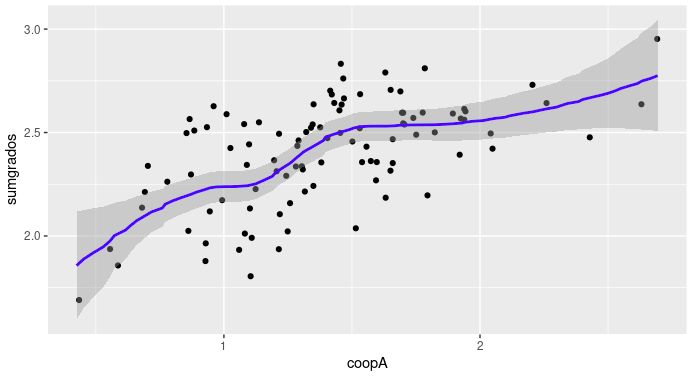
\includegraphics[width=7cm]{img/coopAsum100nonCW}\quad\quad
  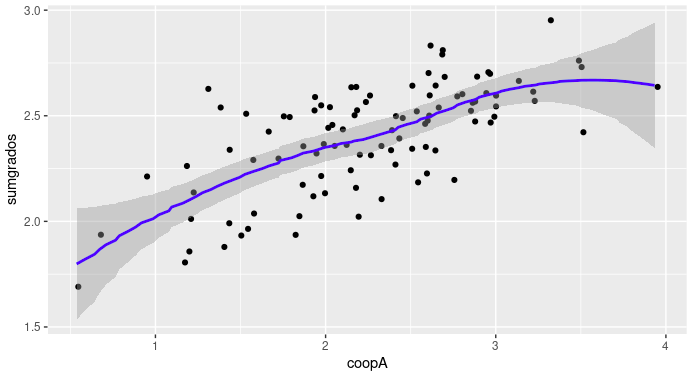
\includegraphics[width=7cm]{img/coopAsumS100nonCW}\\
  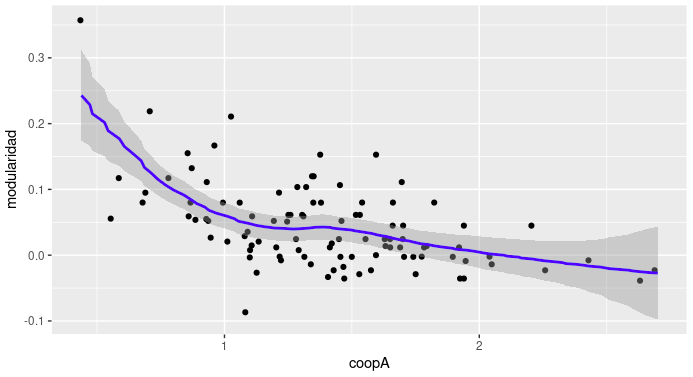
\includegraphics[width=7cm]{img/coopAmod100nonCW}\quad\quad
  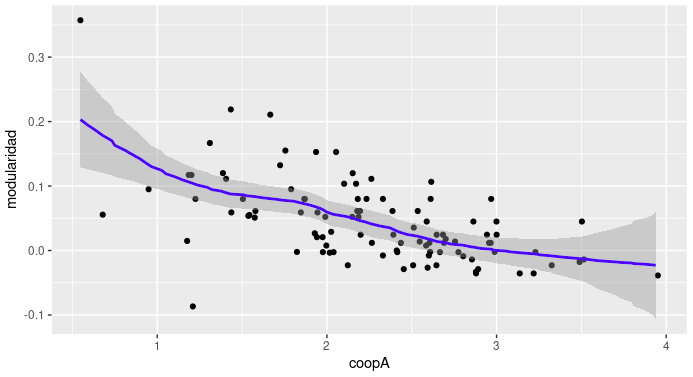
\includegraphics[width=7cm]{img/coopAmodS100nonCW}\\
  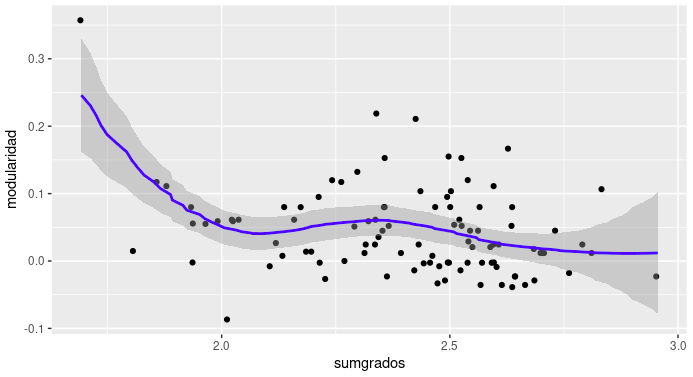
\includegraphics[width=7cm]{img/sumGmod100nonCW}\quad\quad
  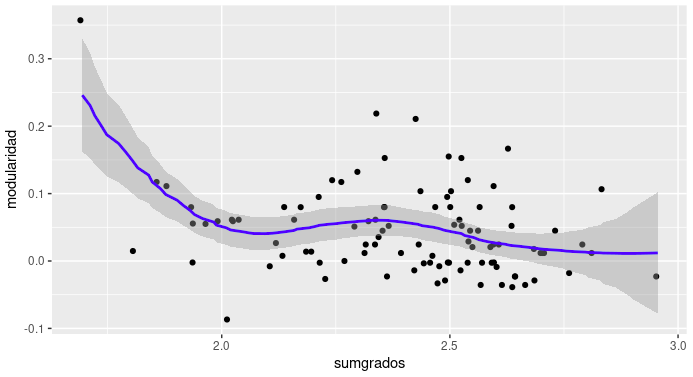
\includegraphics[width=7cm]{img/sumGmodS100nonCW}\\
  \caption{Relation of cooperation value A, modularity and sum of edge
  weights for 100 random graphs. Left: non-symmetric. Right:
  symmetric. Each point corresponds to the average value of the
  measures of a given graph for the 200 random $\alpha$ values.}
  \label{fig:copSumMod100nonCW}
\end{figure}

Relevant correlations appear when looking at the mean of IS and
GR measures for all 200 $\alpha$s in each graph.

Figs.~\ref{fig:corr100nonCW} and~\ref{fig:copSumMod100nonCW} look at
what happens when the sum of weights is different. The greater the
weight is, the greater average cooperation there is in the IS. But
there is also a correlation of cooperation with other measures like
modularity (Fig.~\ref{fig:copSumMod100nonCW}). 

\begin{figure}[htbp!]
  \centering{}
  % Non-symmetric
  % \begin{comment}
  %   chart.Correlation(cor(redes1000group[,c(2,3,4,5,6,8,9,10)],
  %   method="spearman"),2) 
  %   ggplot(data = redes1000group) +
  %   geom_point(mapping = aes(x = coopA, y = modularidad)) +
  %   geom_smooth(mapping = aes(x = coopA, y = modularidad))
  %   ggplot(data = redes1000group) +
  %   geom_point(mapping = aes(x = coopA, y = tamano)) +
  %   geom_smooth(mapping = aes(x = coopA, y = tamano))
  %   ggplot(data = redes1000group) +
  %   geom_point(mapping = aes(x = coopA, y = transitividad)) +
  %   geom_smooth(mapping = aes(x = coopA, y = transitividad))
  %   ggplot(data = redes1000group) +
  %   geom_point(mapping = aes(x = coopA, y = diametroS)) +
  %   geom_smooth(mapping = aes(x = coopA, y = diametroS))
  %   ggplot(data = redes1000group) +
  %   geom_point(mapping = aes(x = coopA, y = Frond)) +
  %   geom_smooth(mapping = aes(x = coopA, y = Frond))
  % \end{comment}
  % Symmetric:
  % \begin{comment}
  %   chart.Correlation(cor(redesS1000group[,c(2,3,4,5,6,8,9,10)],
  %   method="spearman"),2) 
  %   ggplot(data = redesS1000group) +
  %   geom_point(mapping = aes(x = coopA, y = modularidad)) +
  %   geom_smooth(mapping = aes(x = coopA, y = modularidad))
  %   ggplot(data = redesS1000group) +
  %   geom_point(mapping = aes(x = coopA, y = tamano)) +
  %   geom_smooth(mapping = aes(x = coopA, y = tamano))
  %   ggplot(data = redesS1000group) +
  %   geom_point(mapping = aes(x = coopA, y = transitividad)) +
  %   geom_smooth(mapping = aes(x = coopA, y = transitividad))
  %   ggplot(data = redesS1000group) +
  %   geom_point(mapping = aes(x = coopA, y = diametroS)) +
  %   geom_smooth(mapping = aes(x = coopA, y = diametroS))
  %   ggplot(data = redesS1000group) +
  %   geom_point(mapping = aes(x = coopA, y = Frond)) +
  %   geom_smooth(mapping = aes(x = coopA, y = Frond))
  % \end{comment}
  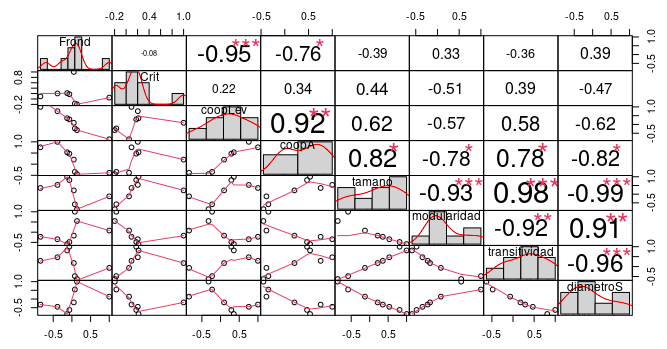
\includegraphics[width=8cm]{img/corr1000group}\quad\quad
  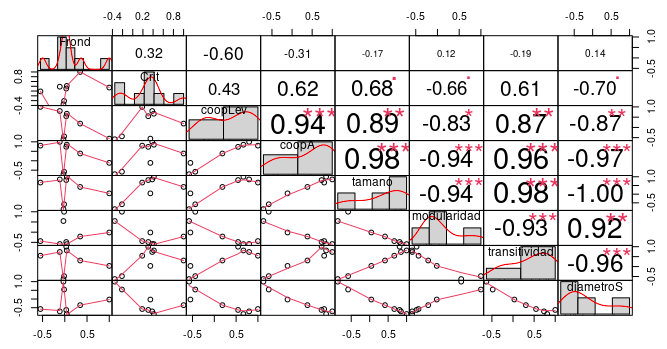
\includegraphics[width=8cm]{img/corrS1000group}
  \caption{Correlation of IS (average for 200 random $\alpha$ values)
    and GR measures in 1000 random graphs. Left: non-symmetric. Right:
    symmetric.}
  \label{fig:corr1000group}
\end{figure}


\begin{figure}[htbp!]
  \centering{}
  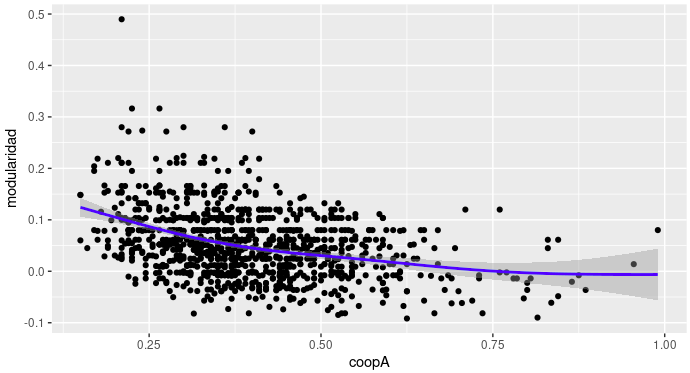
\includegraphics[width=6cm]{img/rel1000groupCoopMod}\quad\quad
  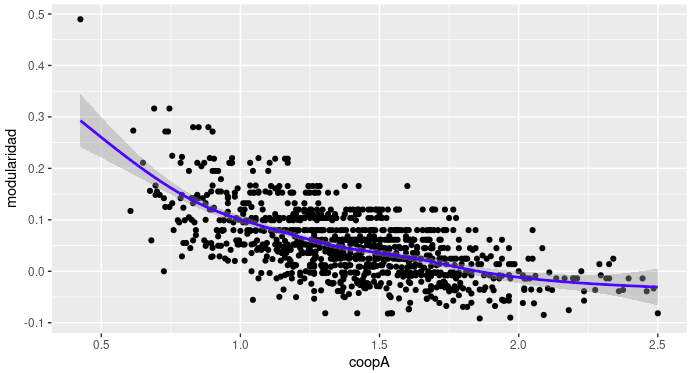
\includegraphics[width=6cm]{img/relS1000groupCoopMod}\\
  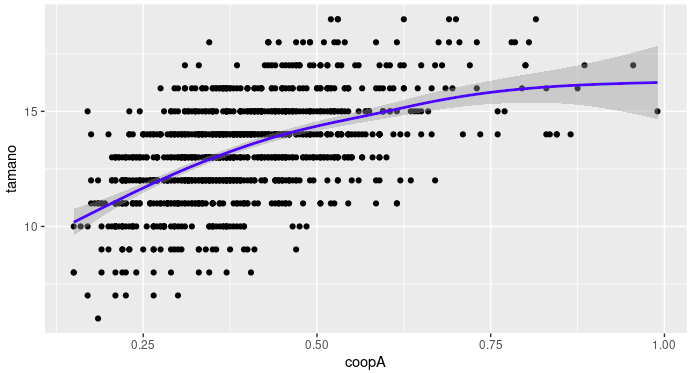
\includegraphics[width=6cm]{img/rel1000groupCoopTam}\quad\quad
  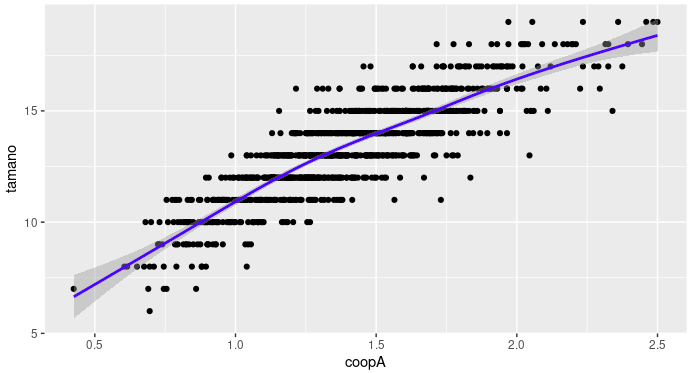
\includegraphics[width=6cm]{img/relS1000groupCoopTam}\\
  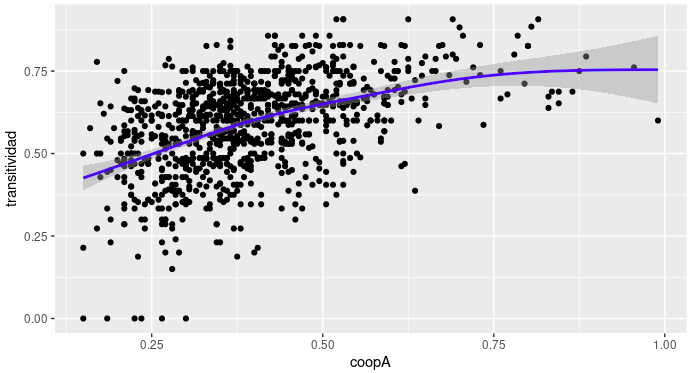
\includegraphics[width=6cm]{img/rel1000groupCoopTrans}\quad\quad
  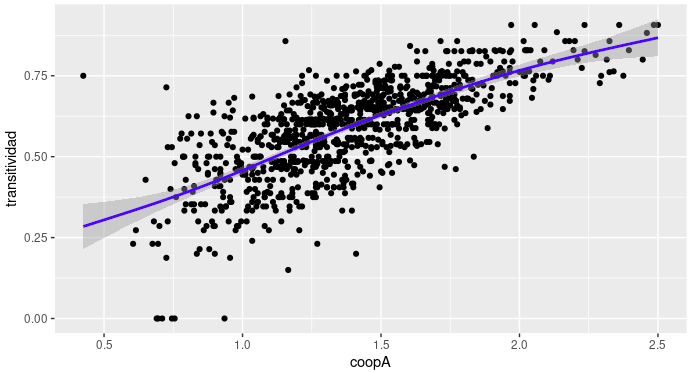
\includegraphics[width=6cm]{img/relS1000groupCoopTrans}\\
  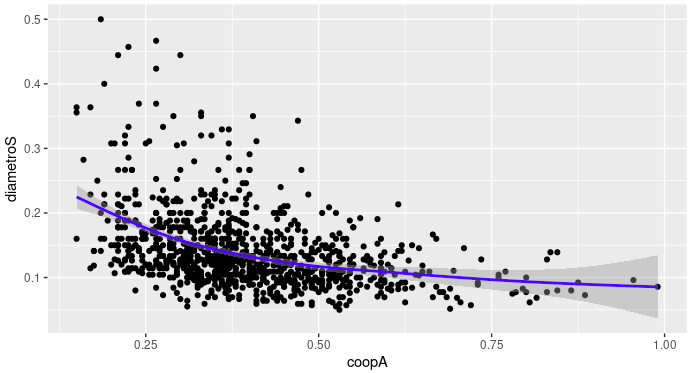
\includegraphics[width=6cm]{img/rel1000groupCoopDiam}\quad\quad
  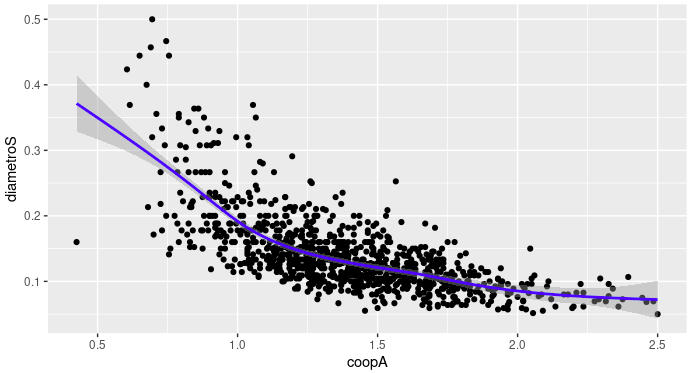
\includegraphics[width=6cm]{img/relS1000groupCoopDiam}\\
  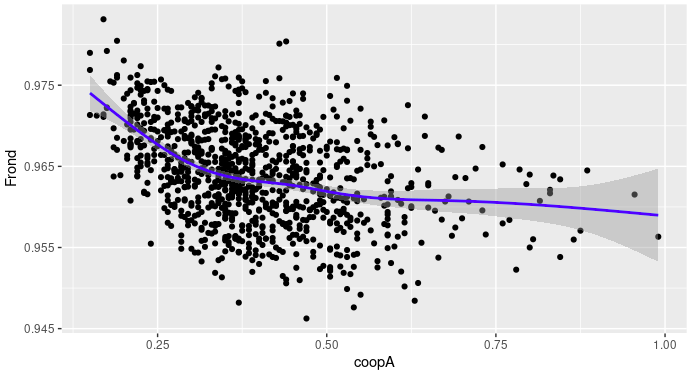
\includegraphics[width=6cm]{img/rel1000groupCoopFrond}\quad\quad
  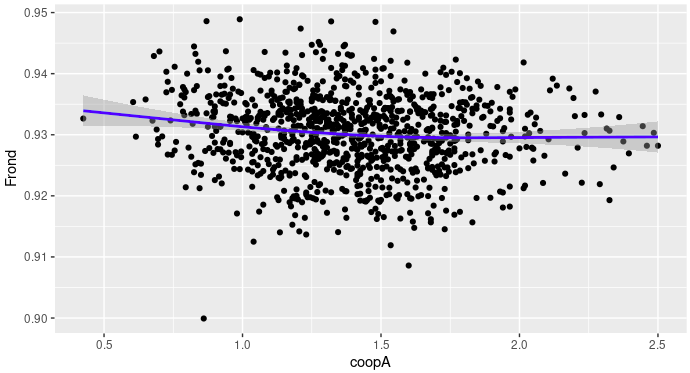
\includegraphics[width=6cm]{img/relS1000groupCoopFrond}
  \caption{Relation of cooperation A value and other measures in
    non-symmetric (left) and symmetric (right) 1000 random graphs. IS
    measures are the average on 200 different $\alpha$ values.}
  \label{fig:coopAndISGR1000}
\end{figure}

To leave aside the effect of having different edge weight, we now look
at the relation of average IS measures with GR parameters by using the
original graphs, all of them with the same sum of edge weights
(Figs.~\ref{fig:corr1000group} and~\ref{fig:coopAndISGR1000}). 


\section{Methods}

\textbf{R}: libraries: \texttt{fitdistrplus} (estudio estadístico de la redes de Web-of-Life para decidir la distribución a utilizar) \texttt{igraph} (graph measures), \texttt{rgraph6} (generacion de grafos)

\section*{TO DO:} 

\begin{enumerate}
    \item look at the relation with structural stability.
Test with some greater graphs
    \item \textbf{diversity}: habría que comprobar si los vértices de grado dos o menos afectan al cálculo, eso no está hecho

\end{enumerate}



\end{document}


